\documentclass[a4paper,12pt]{article}

\usepackage[margin=0.8in]{geometry} % Sets a 0.8 inch margin on all four sides 
\usepackage{parskip} % Block Paragraphs
\usepackage{fancyhdr} % Fancy headers and footers
\usepackage{graphicx} % Enables images
\usepackage{pdfpages} % Embedded PDF files
\usepackage{caption} % Enables captions
\usepackage{mdframed} % Enables frames
\usepackage{verbatim} % Enables insertion of text files
\usepackage{wrapfig} % Wrapped figures
\usepackage{algorithm2e} % Algorithms
\usepackage{tikz} % Drawing
\usepackage{verbatim} % Embed text files
\usepackage[colorlinks=true,urlcolor=blue,linkcolor=blue,linktocpage=true]{hyperref} % Hypertext referencing

\usetikzlibrary{decorations.pathmorphing,calc,shadows.blur,shadings}
\pgfmathsetseed{1} % To have predictable results
% Define a background layer, in which the parchment shape is drawn
\pgfdeclarelayer{background}
\pgfsetlayers{background,main}

% This is the base for the fractal decoration. It takes a random point between the start and end, and
% raises it a random amount, thus transforming a segment into two, connected at that raised point
% This decoration can be applied again to each one of the resulting segments and so on, in a similar
% way of a Koch snowflake.
\pgfdeclaredecoration{irregular fractal line}{init}
{
  \state{init}[width=\pgfdecoratedinputsegmentremainingdistance]
  {
    \pgfpathlineto{\pgfpoint{random*\pgfdecoratedinputsegmentremainingdistance}{(random*\pgfdecorationsegmentamplitude-0.02)*\pgfdecoratedinputsegmentremainingdistance}}
    \pgfpathlineto{\pgfpoint{\pgfdecoratedinputsegmentremainingdistance}{0pt}}
  }
}

% define some styles
\tikzset{
   paper/.style={draw=black!10, blur shadow, shade=bilinear interpolation,
                 lower left=black!20, upper left=black!15, upper right=white, lower right=black!10},
   irregular border/.style={decoration={irregular fractal line, amplitude=0.2},
           decorate,
     },
   ragged border/.style={ decoration={random steps, segment length=7mm, amplitude=2mm},
           decorate,
   }
}

% Macro to draw the shape behind the text, when it fits completly in the
% page
\def\tornpaper#1{
\tikz{
  \node[inner sep=1em] (A) {#1};  % Draw the text of the node
  \begin{pgfonlayer}{background}  % Draw the shape behind
  \fill[paper] % recursively decorate the bottom border
        decorate[irregular border]{decorate{decorate{decorate{decorate[ragged border]{
        ($(A.south east) - (0, random*5mm)$) -- ($(A.south west) - (0, random*5mm)$)
        }}}}}
        -- (A.north west) -- (A.north east) -- cycle;
  \end{pgfonlayer}}
}

\usepackage{amssymb}
\renewcommand{\labelitemi}{\tiny$\blacksquare$} % Black square bullet points

\usepackage{color} % Enables colours
\definecolor{darkpurple}{rgb}{0.4, 0.0, 0.4} % Defines a dark purple colour
\definecolor{javared}{rgb}{0.6,0,0} % for strings
\definecolor{javagreen}{rgb}{0.25,0.5,0.35} % comments
\definecolor{javapurple}{rgb}{0.5,0,0.35} % keywords
\definecolor{javadocblue}{rgb}{0.25,0.35,0.75} % javadoc

\pagestyle{fancy} % Set new page style
\frenchspacing % One space after a full stop
\parindent=0in % Do not indent paragraphs
\brokenpenalty10000\relax % Do not page break at a hyphen

\fancyhf{} % clear all header and footers
\renewcommand{\headrulewidth}{0pt} % remove the header rule
\rfoot{\thepage} 

\usepackage{listings}
  \usepackage{courier}
  \lstloadlanguages{C++}
  \lstset{
         language=C++,
         basicstyle=\footnotesize\ttfamily, 
         numbers=left,               
         numberstyle=\tiny,          
         numbersep=10pt,              
         tabsize=4,                  
         extendedchars=true,         
         breaklines=true,            
    	 frame=lrtb,         
         keywordstyle=\color{javapurple}\bfseries,
         stringstyle=\color{javared},
         commentstyle=\color{javagreen},
         morecomment=[s][\color{javadocblue}]{/**}{*/},
         showspaces=false,           
         showtabs=false,            
         xleftmargin=17pt,
         framexleftmargin=17pt,
         framexrightmargin=5pt,
         framexbottommargin=4pt,
         %backgroundcolor=\color{},
         showstringspaces=false      
 }

\DeclareCaptionFont{white}{\color{white}}
\DeclareCaptionFormat{listing}{\colorbox[cmyk]{0.43, 0.35, 0.35,0.01}{\parbox{\textwidth}{\hspace{15pt}#1#2#3}}}
\captionsetup[lstlisting]{format=listing,labelfont=white,textfont=white, singlelinecheck=false, margin=0pt, font={bf,footnotesize}}

\begin{document}

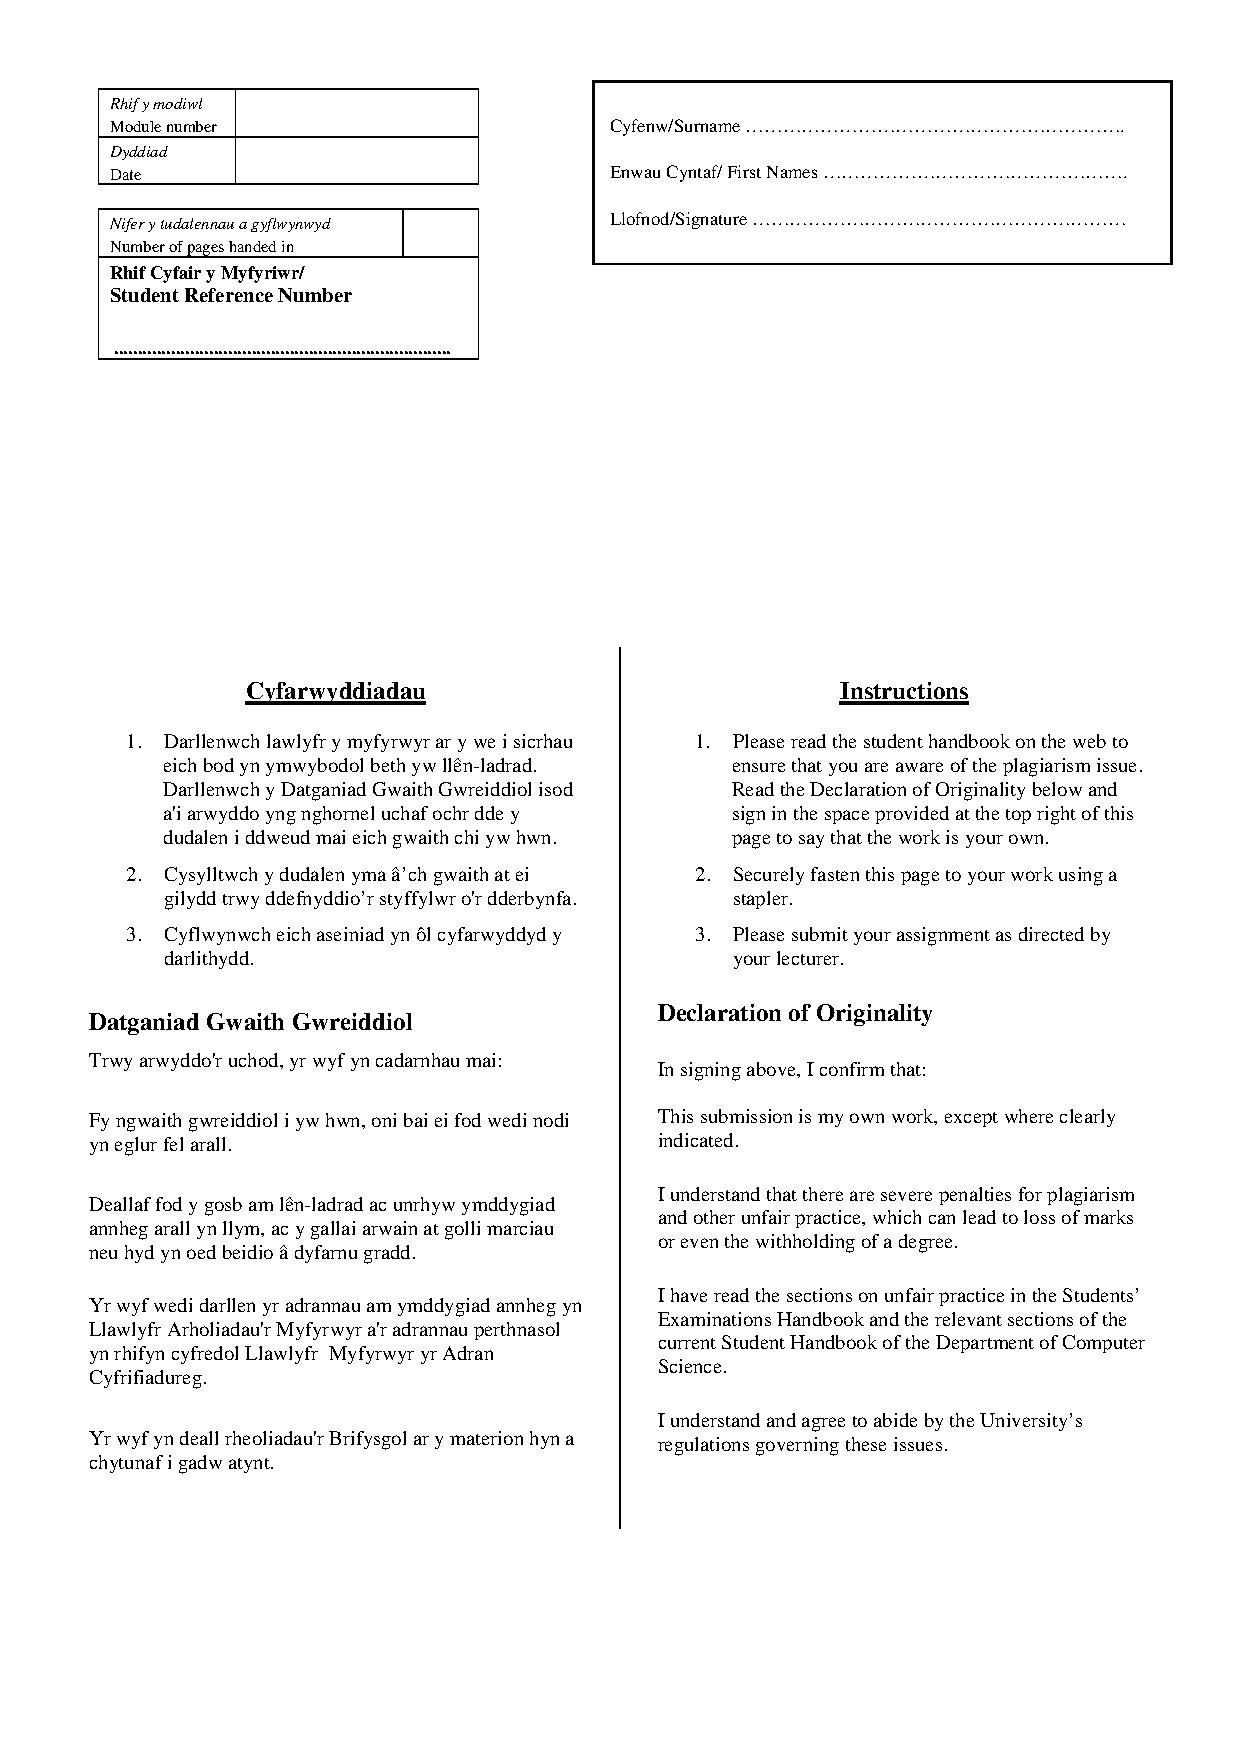
\includepdf{title/assign_cover.pdf} % Coversheet
\includepdf{title/title_page.pdf} % Include title page

\thispagestyle{empty} % Clear page style
\tableofcontents % TOC
\clearpage
\pagenumbering{arabic} % Resets numbering

\section{Introduction}
The purpose of this assignment was to implement a simulated robot to navigate an occupancy grid and then to investigate the differences when this program was used on a real \textit{Pioneer} robot. 

This involved several aspects including navigation, pathfinding, precision movement, navigation and representation of the (simulated or real) environment using appropriate data structures. 

My implementation focused on the following aspects:

\begin{itemize}
    \item{Navigating a simulated occupancy grid}
    \item{Searching for an efficient path using map data as a reference}
    \item{Planning and navigating a given route}
    \item{Versatility in start positions, with the robot regularly recalculating its route}
    \item{Environmental awareness of obstacles, including disallowing illegal goal positions}
\end{itemize}

In addition to this, this program was tested on a real robot and results observed. 

The pathfinding implementation is deliberative as opposed to reactive - my justification for this is that sonars are unnecessary when a full map of the environment is available. However, I familiarised myself with both approaches during the design phase.

Throughout the project, source control was used - both for backup purposes and to provide a record of progress made during the development of my solution.

\scriptsize
\noindent
\tornpaper{
    \parbox{\textwidth}{\verbatiminput{../../Misc/Commit_History.txt}}
}
\normalsize
\newpage
\section{Player/Stage}
\begin{wrapfigure}{r}{0.6\textwidth}
    \begin{center}
            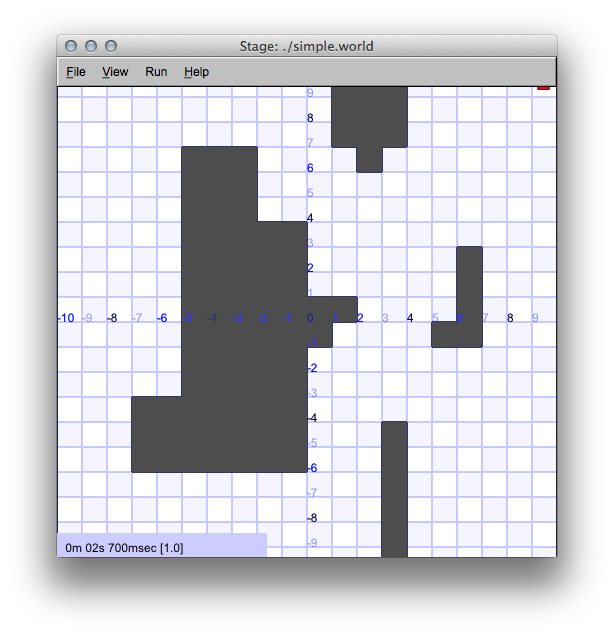
\includegraphics[width=0.6\textwidth]{images/Start_GUI.png}
            \caption{\textit{Player/Stage} Running}
    \end{center}
\end{wrapfigure}
\textit{Player/Stage} is a robotics simulation platform - it combines a simulator (\textit{Stage}) with a client (\textit{Player}) for use when programming robots. 

\textit{Player/Stage} makes use of a TCP based architecture \cite{pstcp} and is therefore network aware. The same code used in the simulator can be executed on a real robot with minor changes, although it may work differently or not at all.

\textit{Player/Stage} proved difficult to install even on the recommended platform (32-bit Linux) and was prone to crashes and graphical glitches such as axes labels disappearing. I installed it from source on \textit{Mac OS X} and it was similarly unreliable. Additionally, there was not much documentation provided and the Java API seemed to have a number of bugs. 

For this reason; as well as personal preference, C\textit{++} was used to implement my navigation system.
\section{Representation}
The first step to solving the issue of navigating the grid was to determine how best to represent states within the program. I decided to use a \textbf{Grid} class to represent the occupancy grid. There was also a need for a \textbf{Node} class to store potential states for use in a graph search. 
\subsection{Grid Class}
The \textbf{Grid} class provides key functionality. It stores the occupancy grid and provides several useful functions to detect obstacles as well as the critically important \texttt{mapToGridArray} function, which converts between $x,y$ coordinates and indices in a two-dimensional \textit{vector} of \textit{int} values. 

This function is crucial, it is used throughout the program whenever a conversion is needed between apparent position on the screen and the internal representation of the environment. This will be discussed further in a later section.
\subsection{Node Class}
The \textbf{Node} class provides all the required functionality to describe a state during navigation. The following table describes the attributes stored in a \textit{Node} object.
\begin{table}[h!]
\scriptsize
\begin{tabular}{|c|c|l|}
    \hline
    \multicolumn{1}{|c|}{\textbf{Attribute}} & \multicolumn{1}{c|}{\textbf{Type}} & \multicolumn{1}{c|}{\textbf{Purpose}} \\
    \hline
    nodeCount & \texttt{static int} & Class-side variable that is updated in the constructor with every new \texttt{Node} instance\\
    \hline
    nodeId & \texttt{int} & Uniquely identifies a Node, increments \texttt{nodeCount} in every new instance\\
    \hline
    parentNode & \texttt{Node*} & Pointer to the parent node, allows tree traversal from leaf to root node \\
    \hline
    gridState & \texttt{Grid} & Instance of a \texttt{Grid},  the current grid state in its entirety\\
    \hline
    pathCost & \texttt{int} & Current path cost, for positions \textit{not} adjacent to obstacles this will be \texttt{parentNode->getPathCost() + 1} \\
    \hline
    xPos & \texttt{int} & Current \textbf{x} coordinate of robot on grid, one part of uniquely identifying a \texttt{Node} \\
    \hline
    yPos & \texttt{int} & Current \textbf{y} coordinate of robot on grid, second part of unique identifier\\
    \hline
    moveDir & \texttt{Direction} & Instance of the \texttt{Direction} enumerated value - see section on graph search \\
    \hline
\end{tabular}
\normalsize
\end{table}

Nodes are created and stored as required, once the path from the start to the goal has been found, The path is reversed and 'replayed' by giving movement commands to the robot sequentially.
\subsection{Occupancy Grid Mapping}
One of the crucial functions required for any movement was the ability to map the robot's apparent position in the simulator to an index in the internal vector. After some experimentation the equation for the position was discovered and the algorithm was implemented. 

Below you can see the basic algorithm, example output to check for correctness and my C\texttt{++} implementation which returns a \texttt{<std::pair>}.

\begin{mdframed}
    \begin{minipage}[t]{.5\textwidth}
            \vspace{0.2cm}
        \small
        \begin{algorithm}[H]
            \DontPrintSemicolon
            \SetAlgoLined
            \KwData{Grid Coordinates of form x,y}
            \KwResult{Indices for position in 2D \textit{vector}}
                \hspace{0.6cm}Let gridX = input x coordinate\\
                \hspace{0.5cm} Let gridY = input y coordinate\\
                \vspace{0.3cm}
                \hspace{0.5cm} Let indexX := $10\:+$ gridX\\
                \hspace{0.5cm} Let indexY := $9\:-$ gridY\\
                \vspace{0.3cm}
                \hspace{0.6cm}\Return indexX, indexY\;
        \end{algorithm}
        \normalsize
    \end{minipage}
    \begin{minipage}[t]{.5\textwidth}
            \small
            \vspace{0.2cm}
            \verbatiminput{/dev/shm/foo.txt}
            \normalsize
    \end{minipage}
\end{mdframed}

\lstset{caption={Mapping Function}}
\begin{lstlisting}
std::pair<int,int> Grid::mapToGridArray(int xPos, int yPos)
{
    std::pair<int,int> arrayPosition;

    arrayPosition.first = 9 - yPos ; // The row
    arrayPosition.second = 10 + xPos; // The column

    /* Returns the 2D vector indices of the given x,y coordinate */
    return arrayPosition; 
}
\end{lstlisting}
\section{Localisation}
Localisation is an important part of robotic navigation, a robot needs to know its current position before it can plan to go anywhere else. The \textit{PositionProxy} class from the API provides several functions to get the current location such as \texttt{GetXPos}. Using these it is possible to obtain the location of the robot.

For higher precision, a \textit{double} can be returned from these functions, otherwise this can be cast to an integer. It is important to update the odometry so that the position of the robot is accurate \textit{before} a path is calculated, or this will lead to errors. 

Reading this data is done by using the \texttt{Read} function provided in the \textit{PlayerClient} class. This should be called regularly to assist with navigation.

The caveat is that the values returned will be estimated at best on a real robot and further calculations will be required to determine how far the robot has moved and its current location.

After the robot moves the internal grid position must also be updated as it is used for the search. This is achieved using the \texttt{moveRobot} function in the \textit{Grid} class. Prior to starting it is also necessary to set the start position of the robot in the grid, this is achieved using the \texttt{setRobotIdx} function. 

The mapping function explained in the previous section is used whenever the position needs to be converted between coordinates and indices.
\section{Reactive and Deliberative Pathfinding}
Robots can be broadly classified into three categories:

\begin{itemize}
    \item{Reactive}
    \item{Deliberative}
    \item{Hybrid}
\end{itemize}
When designing this software it was important to consider the advantages and disadvantages of each of these approaches. 

Reactive robotics is based on a direct mapping between sensors and output and focuses on being fast and uncomplicated. This approach may provide similar results in the simulator as it does on the real robot because it does not require an internal representation of the environment, it reacts to obstacles as they appear.

The way to perform this sort of reactive pathing on the \textit{Pioneer} is through the use of sonars.

Deliberative robotics uses planning and constructs an internal representation of the environment which can be manipulated internally before the robot moves. The typical way a deliberative pathfinder works would be to look ahead using AI search techniques (commonly \textit{A*} or \textit{Best First} Search) and calculate the route needed to get from the start position to the goal position without colliding with any obstacles.

This approach is ideal when obstacles are static and the movement is not time-critical, allowing time for calculating an ideal route. As obstacles on the provided occupancy grid do not move, this navigation method could prove very effective. There is also potential for the search to be more dynamic by recalculating the path should the robot be moved or come near obstacles.

Representation could prove troublesome because the robot will have to represent positions, obstacles and so forth as abstractions. This is in contrast to the reactive approach which uses the "world as its own best model" approach. Another potential difficulty is the need to keep the internal model synchronised with the robots movements in the simulated or real environment.

Hybrid robotics would involve a combination of both navigational techniques. This would appear to be ideal and would involve constructing a map using sonar data as a dynamic input.
\subsection{Sonar}
\begin{wrapfigure}{r}{0.5\textwidth}
    \begin{center}
            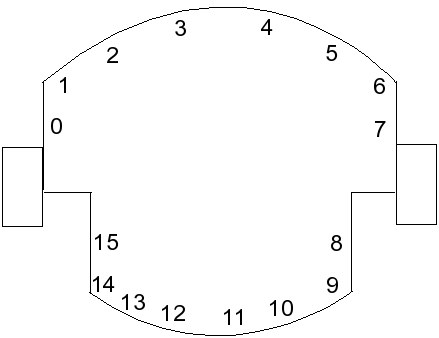
\includegraphics[width=0.47\textwidth]{images/sonars_wiki_dcs_aber_ac_uk.png}
            \caption{Layout of sonars on the \textit{Pioneer} \cite{sonardiagram}}
    \end{center}
\end{wrapfigure}

The \textit{Pioneer} robot has an array of between eight and sixteen sonars which allow for obstacle detection.

These are potentially more effective in the simulator as they are not at risk of cross-talk or environmental factors. 

If two sonar equipped robots are near each other then their sonar readings could be responding to the sonar outputs from the other robots and cause issues.

Sonars are easy to use in the provided C++ API via a \texttt{RangerProxy} or \texttt{SonarProxy} for simulation or real environments respectively. 

Sonars are indexed from $0-15$ and can be accessed using standard array notation.

\lstset{caption={Example Sonar Handling}, mathescape=true}
\begin{lstlisting}
if (rp[3] < 1 || rp[4] < 1) // An object is detected in front of the robot
{
    pp.SetSpeed(-0.700, dtor(60)); // Move backwards whilst turning 60 deg.
    usleep(300000); // Hold movement for 3 seconds
} 
\end{lstlisting}
\subsection{Graph Search}
As mentioned in the previous section, a graph search is an effective navigation method when obstacles remain stationary. A graph search requires the following:
\begin{itemize}
    \item{State space}
    \item{Initial state}
    \item{Goal state}
    \item{Successor function / Operators}
    \item{Restrictions}
    \item{Solution}
\end{itemize}

The state space for the occupancy grid is every potential (legal) position the robot could occupy. The initial state is the hard-coded occupancy grid and the goal state is defined by the user.
\begin{wrapfigure}{l}{0.5\textwidth}
    \begin{center}
            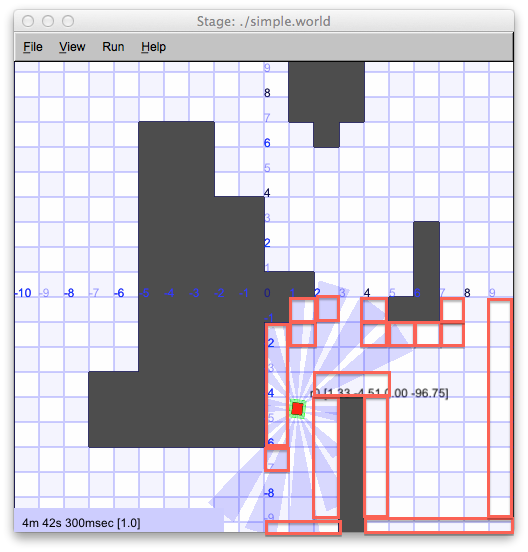
\includegraphics[width=0.47\textwidth]{images/Path_Cost_Grid.png}
            \caption{Higher cost positions in this quadrant are marked in orange}
    \end{center}
\end{wrapfigure}

The successor function creates new nodes with a direction of movement (Up, Down, Left, Right) and sets variables for these nodes (e.g. current path cost, current grid state) accordingly. Operators for changing state can be surmised as moving in one of the four directions from the current position. 

Restrictions are implemented in an \textit{A*} search with path cost and in all searches by only allowing legal positions for successor nodes. There are several functions related to checking for legal moves which can also be used for input validation.

The \textit{Grid} class has three related functions these are \texttt{canMove}, \texttt{isObstacle} and \texttt{adjacentToObstacle} - the first of these functions takes a grid coordinate, converts it to an index value and then returns true if either the robot or an obstacle are occupying that position.

\texttt{adjacentToObstacle} checks a given grid coordinate and returns true if it is adjacent to an obstacle in any direction. In order to have the search prioritise non-adjacent positions (to prevent getting too close to obstacles) these are given a higher path cost. This 'dissuades' the robot visiting these positions unless one of them is a goal position.

\lstset{caption={\texttt{adjacentToObstacle} function, checks in eight directions}}
\begin{lstlisting}
bool Grid::adjacentToObstacle(int xPos, int yPos)
{
    if (xPos == GRID_MIN_X || xPos == GRID_MAX_X || yPos == GRID_MIN_Y || yPos == GRID_MAX_Y) { // Edge of grid counts as obstacle
        return true;
    }

    if (isObstacle(xPos + 1, yPos) || isObstacle(xPos - 1, yPos) || isObstacle(xPos, yPos + 1) || isObstacle(xPos, yPos - 1)) {
        return true;
    }

    /* Check diagonally for obstacles */
    if (isObstacle(xPos +1, yPos + 1) || isObstacle(xPos -1, yPos - 1) || isObstacle (xPos - 1, yPos + 1) || isObstacle(xPos + 1, yPos - 1)) {
        return true;
    }

    return false;
}
\end{lstlisting}

The solution is presented as a sequence of coordinates to travel along, these can be 'replayed' by the robot by reversing the path from the goal node to the root node, allowing it to move along the calculated path.
\section{Development}
Over the course of development, my ideas changed quite significantly and the final software was a lot different to the original version. This is unsurprising and proved useful in terms of seeing how my ideas had developed. 

In the following two sections I discuss alternatives I tried and the process of developing the final software implementation.
\subsection{Early Ideas}
Early on in the development process I looked at using a very crude reactive approach by simply having the robot check sonars and randomly move about the environment. This was effective but did not involve any intelligent motion or significant robotics knowledge. 

I discovered that the \textit{Player/Stage} API provided a \texttt{GoTo} function as a member of the \texttt{PositionProxy} class. This function would allow me to input a position using the \texttt{player2d\_pose\_t} type (a simple pair like structure) and from there the robot would navigate to this position on the grid.

This seemed like a very simple solution - avoid obstacles with the sonar and move towards the goal position. After running some tests I concluded that the \texttt{GoTo} function was not intelligent and would simply move to the position in a straight line. I also discovered that movement commands sent to the robot are executed continually until a new command is received.

What this meant was that I would have to repeatedly send \texttt{GoTo} commands and pause for the sonar data to be read, very inelegant. Because there was no intelligence the robot would often come too close to obstacles and get stuck when trying to turn or become caught in a loop where it moved towards an obstacle, backed away and moved towards it again.

It was clear I would need to try a different approach. I discovered that the \texttt{usleep} function provided in \textit{cstdlib} would allow commands sent to the robot to be carried out for a length of time before the new command was sent - this seemed useful but did not prevent issues where a robot would move towards an obstacle, and be sleeping whilst the sonar should have been picking up new data and sending an avoidance command.

This could have been fixed by implementing some sort of threading capability or using an interrupt but continuing on this path seemed less about intelligent robotics and more about exploiting C\texttt{++} features, so I decided to drop the idea of a reactive system and try a deliberative one.

I began by attempting to implement a simple breadth-first search which required the creation of a \textit{Node} class. I moved everything around in memory without sending commands to the robot yet in order to see if this was feasible. 

I had some initial difficulty because I didn't realise I needed to use pointers to \textit{Node} objects rather than \textit{Node} objects themselves in my data structures. When I was storing \textit{Node} objects the \texttt{getParentNode} function was not working correctly. This is crucial for tree traversal, an example of which follows:

\lstset{caption={Tree traversal example}}
\begin{lstlisting}
 for (Node* n : explored)
    {
        if (n->isGoalState(goalX, goalY)) // Found the node which represents the goal state
        {
            while (n->getParentNode() != NULL) // Traverse upwards until we reach the root node 
            {
                pathString.append(n->getMoveDirString()); // Append the direction to the output string
                calculatedPath->push_back(n); // Add the node to the path the robot will take
                n = n->getParentNode(); // Move one level back up the tree
            }
        }
    }
    std::reverse(pathString.begin(), pathString.end()); // Reverse the string so it displays start -> goal instead of vice-versa
    std::cout << "\n\nPATH: " << pathString << std::endl;

    std::reverse(calculatedPath->begin(), calculatedPath->end()); // Reverse vector storing the path in a similar mannner
\end{lstlisting}

This worked well and I decided to continue with the deliberative approach, however the breadth-first search proved extremely slow when calculating positions that were further away from the robot than the local quadrant.
\subsection{Final Implementation}
To solve the problem of breadth-first search being too slow, I added a heuristic and modified it into a best-first search. This greatly improved the performance, although I ran into issues with some coordinates because my check to see if a node was already in the explored list was failing, again an issue with pointers. I created the following function to dereference the pointers and check the values of the two variables that held position data. Before I did this the search was getting stuck in an infinite loop.

\lstset{caption={Check if node has already been explored}}
\begin{lstlisting}
bool nodeExplored(Node* successorNode)
{
    std::vector<Node*>::iterator it; // Create iterator for Node* container 

    for ( it = explored.begin(); it != explored.end(); ++it)
    {
        if ( (*it)->getXPos() == successorNode->getXPos() && (*it)->getYPos() == successorNode->getYPos())
        {
            return true;
        }
    }
}
\end{lstlisting}

This solved the issue with some goal positions not working but I then had the issue of the robot hitting obstacles regularly. This was because it would move to positions directly adjacent to obstacles, then collide with the obstacles when turning. 

In order to stop this from happening I had to implement a path cost system (as explained in section 5.2) to give those positions lower priority unless one of them was a goal state. The key component of the path cost calculations are whether or not a cell is next to an obstacle (in any of eight directions),

An \textit{A*} search is based on a \textit{priority queue} data structure which allows for the most desirable nodes to be evaluated first. My comparator for the priority queue used in my program is as follows:

\lstset{caption={Priority Queue Comparator}}
\begin{lstlisting}
struct findBestNode : public std::binary_function<Node*, Node*, bool>
{
    bool operator() (const Node* firstNode, const Node* secondNode) const // Overload () operator
    {
        if (distanceFromGoal(firstNode->getXPos(),firstNode->getYPos()) + firstNode->getPathCost() < 
                distanceFromGoal(secondNode->getXPos(), secondNode->getYPos()) + secondNode->getPathCost())
        {
            return false;
        }

        return true;
    }
};
\end{lstlisting}

\textit{A*} search was the only algorithm which worked successfully. For optimal navigation both a path cost and a heuristic are required so breadth-first and best-first search proved inadequate.

Another consideration was the function to check if a goal state had been reached. I realised I had to lower the precision on the \texttt{isGoal} function because the robot would try to move directly to the outer edge of the requested grid cell and could then hit an obstacle. It now stops closer to the centre of the cell at the goal position.

\section{Testing}
When testing this software, I attempted to try a variety of different start and end positions. I tested moving the robot whilst it was navigating and found that it recalculated the path to the goal correctly. 

As well as this,  I tested obstacle avoidance and pathfinding for several different areas of the grid and received generally positive results.

Below is a short test table of the test conducted, any input given and the expected result.
\begin{table}[ht!]
\scriptsize
    \begin{tabular}{|l|c|l|l|}
        \hline
        \multicolumn{1}{|c|}{\textbf{Test Description}} & \multicolumn{1}{c|}{\textbf{Input}}& \multicolumn{1}{c|}{\textbf{Expected Result}} & \multicolumn{1}{c|}{\textbf{Result}} \\
        \hline
        Input coordinate(s) off grid & -12,4 & Output error message and ask user to re-input & PASS\\
        \hline
        Illegal coordinate(s) are obstacles & 5,-1 & Program will output error message and ask user to re-input & PASS\\
        \hline
        Move from start to goal in same quadrant & A: 9,9 B: 4,4 & Robot will reach \textit{B} successfully without hitting obstacles & PASS\\
        \hline
        Move from start to goal in different quadrant & A: -8,-8 B: 4,-3 & Same as above & PASS$^*$\\
        \hline
        Drag robot whilst moving to position & N/A & Robot will recalculate path, displayed in terminal & PASS\\
        \hline
        Goal recognition & Goal position & Robot will stop when approaching goal state & PASS$^*$\\
        \hline
    \end{tabular}
    \\
$^*$ Navigation to different quadrants and goal recognition occasionally display issues, see overleaf.
\normalsize
\end{table}

\newpage
    \begin{figure}
        \begin{center}
            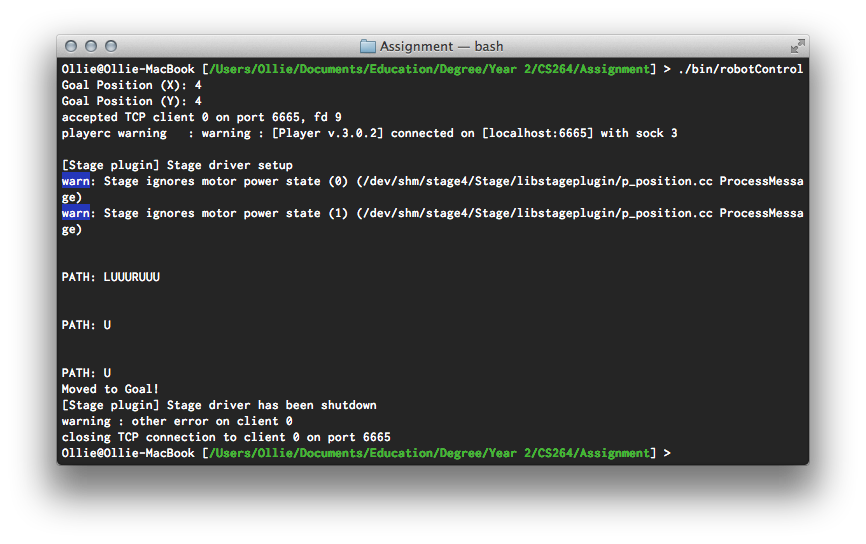
\includegraphics[scale=0.6]{images/Testing_CLI.png}
            \caption{Command line output when moving the robot from \textbf{4,-3} to \textbf{4,4}}
        \end{center}
\end{figure}

From these results, I was able to draw several conclusions about how effective the software is at navigating the occupancy grid:

\begin{enumerate}
    \item{The robot moves to the destination successfully in most cases}
    \item{Occasionally the robot will bump into an obstacle and then correct its course}
    \item{One time out of eight test runs the robot hit an obstacle and was not able to correct its course}
    \item{If a robot is moved during the process of navigation it can successfully renegotiate a path. Localisation works well}
    \item{The robot is able to recognise goal states and stop with high reliability}
    \item{Occasionally the robot will reach the goal state and player will crash with an uncaught exception of type \texttt{PlayerCc::PlayerError}. This is not reproducible}
    \item{The robot occasionally hesitates when running the simulation at normal speed if the goal is a node with lower path cost (i.e. adjacent to an obstacle)}
\end{enumerate}

Testing indicates that the software generally works well, with potential calibration needed in terms of path cost and further obstacle avoidance. In most test cases; the robot was able to navigate the occupancy grid without issue, so the testing was a success overall. The testing also highlighted some apparent deficiencies in \textit{Player/Stage}.

\section{Real Robots}
\begin{figure}[h!]
\begin{center}
    \frame{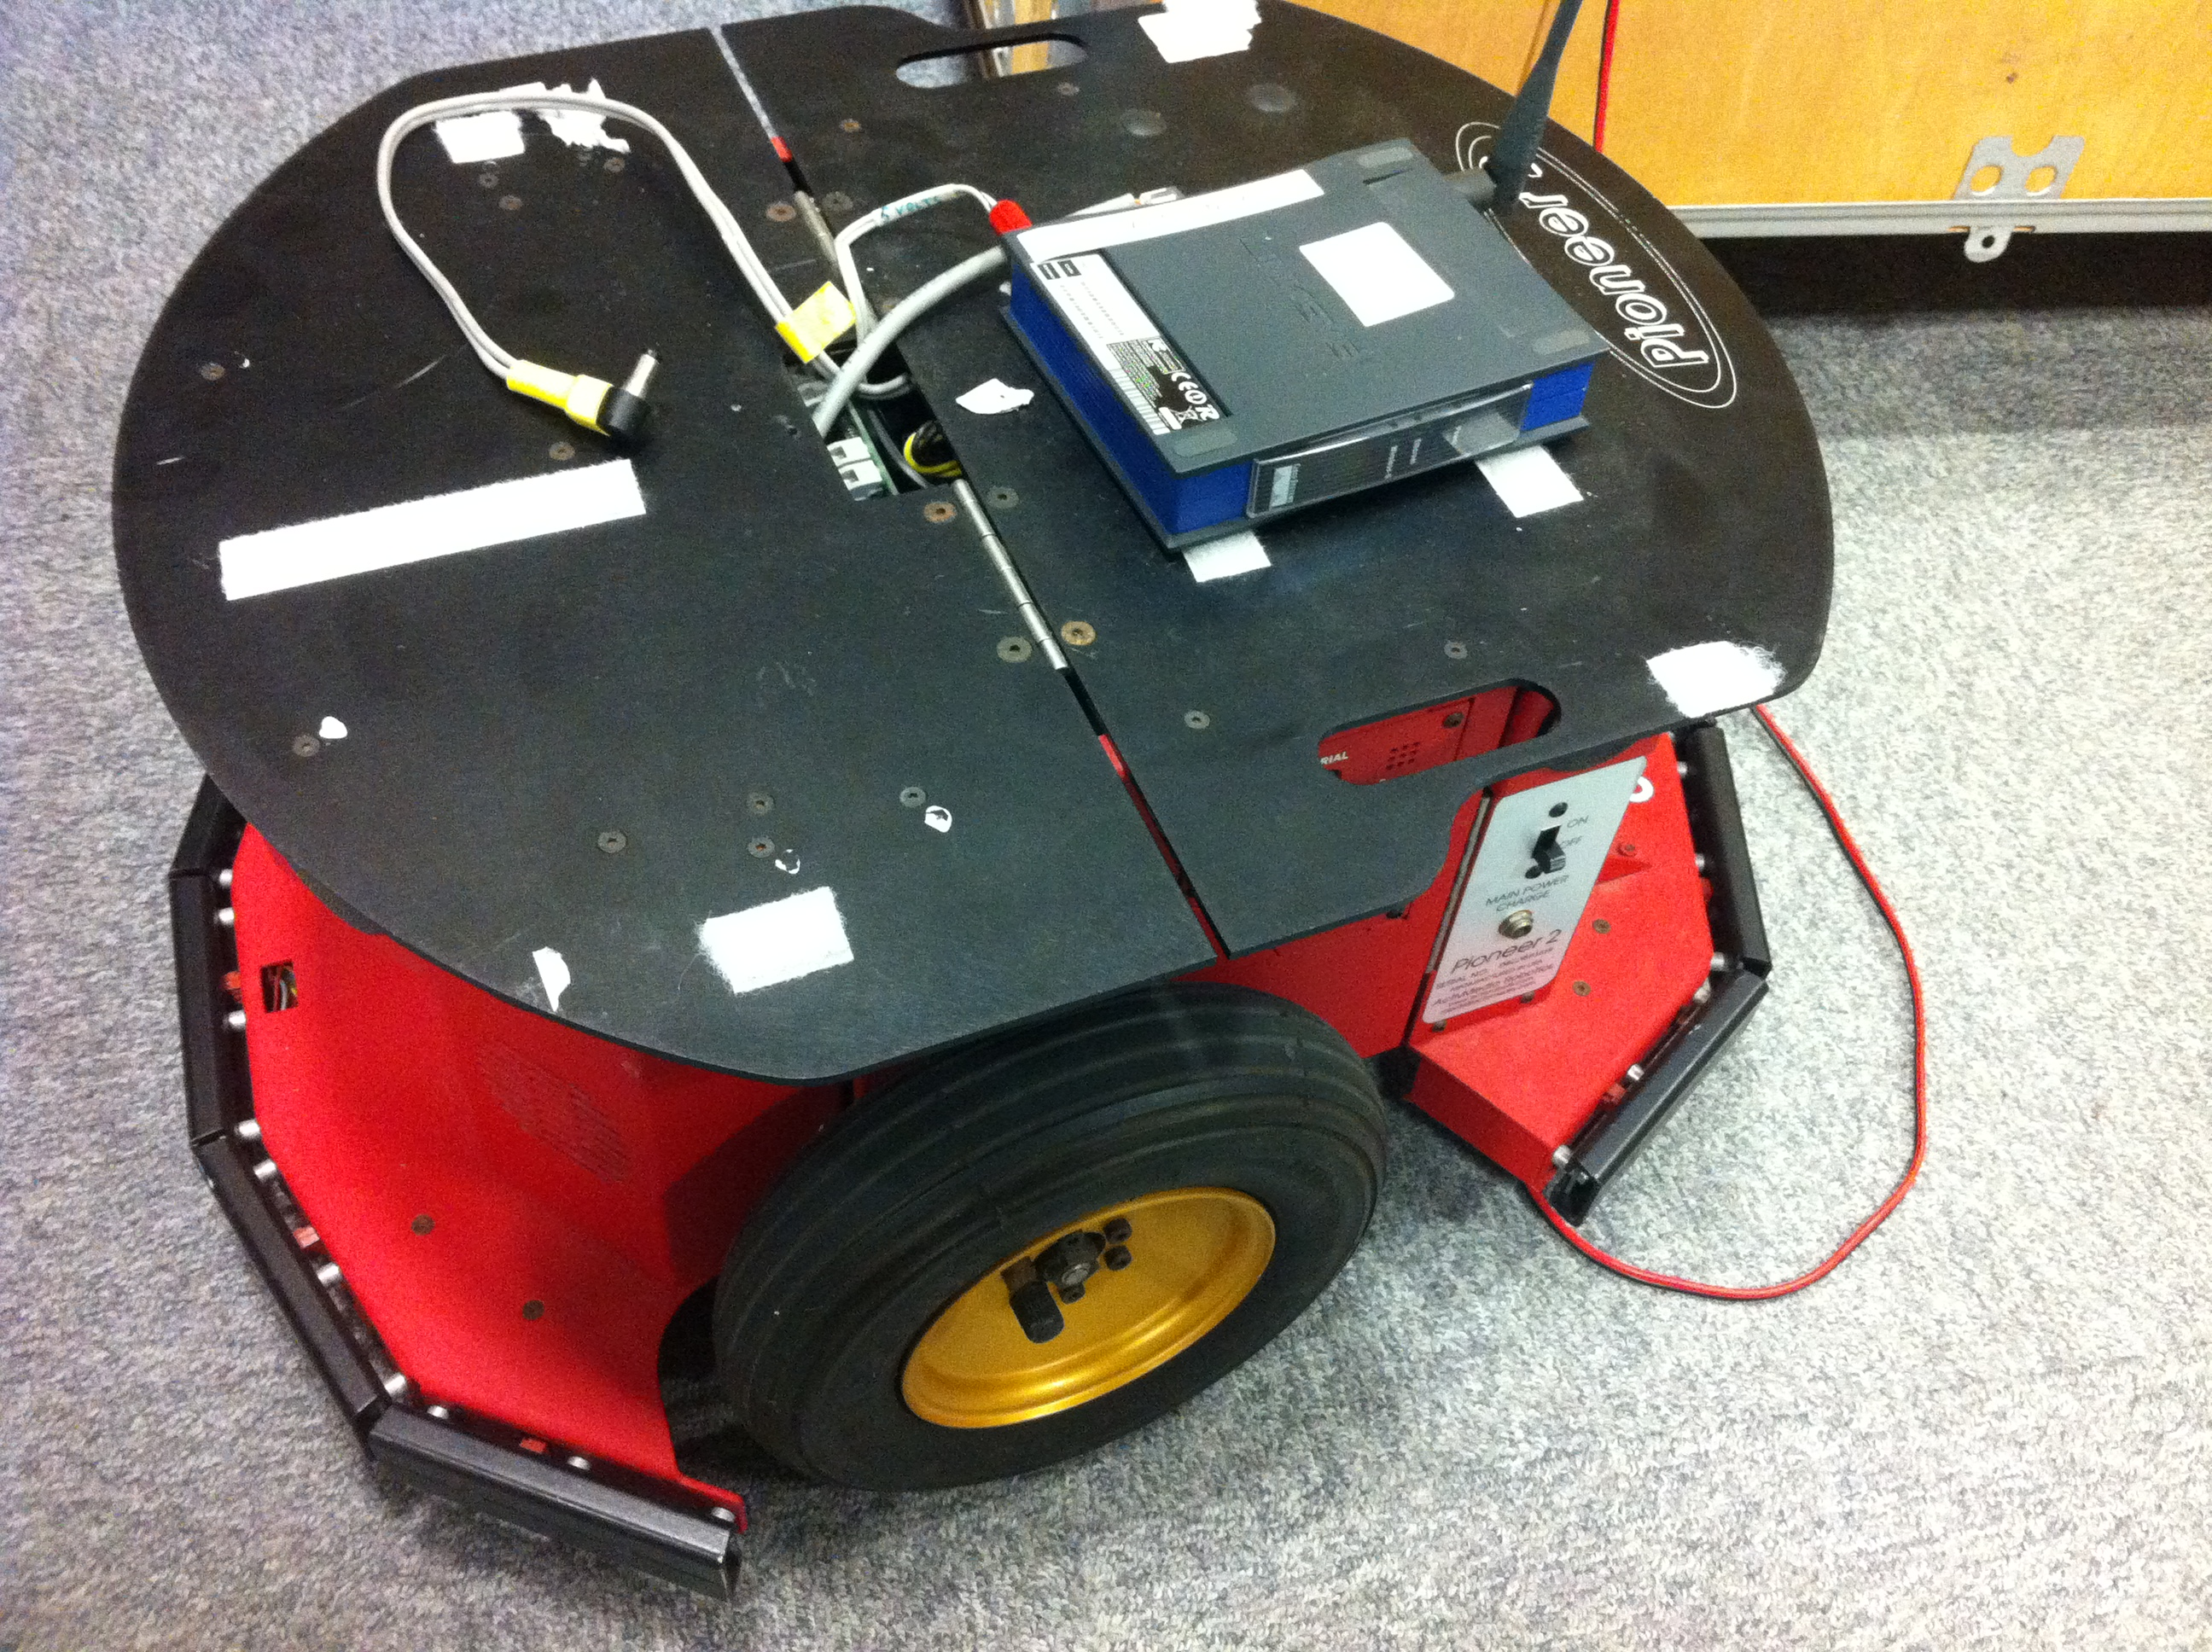
\includegraphics[width=1\textwidth]{./images/Pioneer.jpg}}
    \caption{Pioneer Robot in the Intelligent Systems Laboratory (\textit{ISL})}
\end{center}
\end{figure}
One of the most important parts of this assignment was to try the software on an actual \textit{Pioneer}. As my final implementation was heavily deliberative and the lab environment did not match the provided occupancy grid, I was expecting undefined behaviour. Because I did not make use of the sonars in my final implementation - any behaviour would be avoiding obstacles by chance.

In order to use the sonars I would need to create a local map using provided sonar data. This would not be too difficult as the functionality for setting and creating maps has already been implemented.

I conducted two trials in the lab, the first was a run of my software with no modifications other than changing the \texttt{RangerProxy} to a \texttt{SonarProxy} as required. When executed, my software reacted normally until I had entered start and goal positions and then the robot proceeded to sit without moving. 

On further investigation it appeared that the GoTo command I had based my solution on was not being executed by the robot. The command window stated that path planning was taking place but the robot was immobile. I experimented by manually setting the speed but it was clear that the software would need non-trivial adaptation to use on a real robot. Conceptually the navigation would work but it would be more difficult to ascertain positions, distances and so forth.

The second trial involved running some simple sonar avoidance code to investigate how the robot moved. The main differences in terms of the real robot were as follows:

\begin{itemize}
    \item{Movement is a lot less precise in the simulator. Robots require a turn radius of about $1.5\times$ their length which is less apparent in the simulator }
    \item{\texttt{GoTo} commands mean nothing to an actual robot}
    \item{Real robots take longer to execute commands in general, this would have to be accounted for in a real robotic solution}
    \item{Real robots must respect the laws of physics and their movement parameters such as speed and turn-rate need to be carefully adjusted}
\end{itemize}

\section{Conclusions}
Overall this project proved quite challenging because applying AI techniques to the environment is not as 'clean' as it is when dealing with a structure that exists only in memory. 

Originally the assignment seemed conceptually easy but implementation was less simple, a lot of complexity exists in robotic navigation that I did not understand before taking this assignment on. It was also interesting to see how different the simulator was from real life, prior to testing I expected the \textit{Pioneer} to display \textit{some} of the intended behaviour.

It was interesting how the architecture of the robot differed from a traditional program, in a standard C\texttt{++} program there is no buffer if you are not inside a loop of some kind, commands are only executed once. On the \textit{Pioneer} a movement command is executed until the next movement command is received. This highlights the importance of the \texttt{usleep} commands used to delay the execution of the next command until the previous one has finished.

The software would need modifications to work correctly on a real robot, however the framework for path planning is complete and works well. In order for the robot to navigate arbitrary environments there would need to be a way to convert sonar data into an internal map as well as measure position and speed in a reliable way. 

There are a few bugs in my implementation but nothing which detracts from the ability to navigate the occupancy grid successfully. As mentioned in the previous section, the robot will sometimes stop just short of the goal with a \texttt{PlayrCc::PlayerError} exception - I have not ascertained whether this is a bug with my software or something else as the same error is thrown when the software cannot connect to the server.

Additionally, as soon as the \texttt{PositionProxy} object is instantiated, the \textbf{simulated} robot will begin to move. In order to make the robot wait for input I don't instantiate the \texttt{PositionProxy} until after the user has input the goal coordinates. 

This causes a crash if the coordinates input by the user are the same as the robot's current coordinates, there is no way of checking because \texttt{getXPos} and related functions are not available yet. 

To make the robot wait for input before moving, I could send commands to make the robot move in a tight circle - effectively immobilising it. However the real robot does not exhibit this problem due to \texttt{setMotorEnable(false)} being called so it is not a serious issue.

It has been a valuable learning experience and I now have a much better understanding of robotic navigation and related concepts.
\begin{thebibliography}{10}
    \bibitem{sonardiagram}
    Aberystwyth University DCS. \textit{"Pioneer Robot Sonar Diagram"}, wiki.dcs.aber.ac.uk. [Online]. Available:\\ \url{http://wiki.dcs.aber.ac.uk/doku.php?id=robotics:pioneer_information} [Accessed: Mar. 21 2014].

    \bibitem{pstcp}
    Sourceforge. \textit{"Player/Stage"}, playerstage.sourceforge.net [Online]. Available:\\ \url{http://playerstage.sourceforge.net/player/player.html} [Accessed: Mar. 22 2014].
    \end{thebibliography}

\end{document}

